% Options for packages loaded elsewhere
% Options for packages loaded elsewhere
\PassOptionsToPackage{unicode}{hyperref}
\PassOptionsToPackage{hyphens}{url}
\PassOptionsToPackage{dvipsnames,svgnames,x11names}{xcolor}
%
\documentclass[
]{ctexart}
\usepackage{xcolor}
\usepackage{amsmath,amssymb}
\setcounter{secnumdepth}{5}
\usepackage{iftex}
\ifPDFTeX
  \usepackage[T1]{fontenc}
  \usepackage[utf8]{inputenc}
  \usepackage{textcomp} % provide euro and other symbols
\else % if luatex or xetex
  \usepackage{unicode-math} % this also loads fontspec
  \defaultfontfeatures{Scale=MatchLowercase}
  \defaultfontfeatures[\rmfamily]{Ligatures=TeX,Scale=1}
\fi
\usepackage{lmodern}
\ifPDFTeX\else
  % xetex/luatex font selection
\fi
% Use upquote if available, for straight quotes in verbatim environments
\IfFileExists{upquote.sty}{\usepackage{upquote}}{}
\IfFileExists{microtype.sty}{% use microtype if available
  \usepackage[]{microtype}
  \UseMicrotypeSet[protrusion]{basicmath} % disable protrusion for tt fonts
}{}
\makeatletter
\@ifundefined{KOMAClassName}{% if non-KOMA class
  \IfFileExists{parskip.sty}{%
    \usepackage{parskip}
  }{% else
    \setlength{\parindent}{0pt}
    \setlength{\parskip}{6pt plus 2pt minus 1pt}}
}{% if KOMA class
  \KOMAoptions{parskip=half}}
\makeatother
% Make \paragraph and \subparagraph free-standing
\makeatletter
\ifx\paragraph\undefined\else
  \let\oldparagraph\paragraph
  \renewcommand{\paragraph}{
    \@ifstar
      \xxxParagraphStar
      \xxxParagraphNoStar
  }
  \newcommand{\xxxParagraphStar}[1]{\oldparagraph*{#1}\mbox{}}
  \newcommand{\xxxParagraphNoStar}[1]{\oldparagraph{#1}\mbox{}}
\fi
\ifx\subparagraph\undefined\else
  \let\oldsubparagraph\subparagraph
  \renewcommand{\subparagraph}{
    \@ifstar
      \xxxSubParagraphStar
      \xxxSubParagraphNoStar
  }
  \newcommand{\xxxSubParagraphStar}[1]{\oldsubparagraph*{#1}\mbox{}}
  \newcommand{\xxxSubParagraphNoStar}[1]{\oldsubparagraph{#1}\mbox{}}
\fi
\makeatother


\usepackage{longtable,booktabs,array}
\newcounter{none} % for unnumbered tables
\usepackage{calc} % for calculating minipage widths
% Correct order of tables after \paragraph or \subparagraph
\usepackage{etoolbox}
\makeatletter
\patchcmd\longtable{\par}{\if@noskipsec\mbox{}\fi\par}{}{}
\makeatother
% Allow footnotes in longtable head/foot
\IfFileExists{footnotehyper.sty}{\usepackage{footnotehyper}}{\usepackage{footnote}}
\makesavenoteenv{longtable}
\usepackage{graphicx}
\makeatletter
\newsavebox\pandoc@box
\newcommand*\pandocbounded[1]{% scales image to fit in text height/width
  \sbox\pandoc@box{#1}%
  \Gscale@div\@tempa{\textheight}{\dimexpr\ht\pandoc@box+\dp\pandoc@box\relax}%
  \Gscale@div\@tempb{\linewidth}{\wd\pandoc@box}%
  \ifdim\@tempb\p@<\@tempa\p@\let\@tempa\@tempb\fi% select the smaller of both
  \ifdim\@tempa\p@<\p@\scalebox{\@tempa}{\usebox\pandoc@box}%
  \else\usebox{\pandoc@box}%
  \fi%
}
% Set default figure placement to htbp
\def\fps@figure{htbp}
\makeatother

\ifLuaTeX
  \usepackage{luacolor}
  \usepackage[soul]{lua-ul}
\else
  \usepackage{soul}
\fi




\setlength{\emergencystretch}{3em} % prevent overfull lines

\providecommand{\tightlist}{%
  \setlength{\itemsep}{0pt}\setlength{\parskip}{0pt}}



 


\makeatletter
\@ifpackageloaded{tcolorbox}{}{\usepackage[skins,breakable]{tcolorbox}}
\@ifpackageloaded{fontawesome5}{}{\usepackage{fontawesome5}}
\definecolor{quarto-callout-color}{HTML}{909090}
\definecolor{quarto-callout-note-color}{HTML}{0758E5}
\definecolor{quarto-callout-important-color}{HTML}{CC1914}
\definecolor{quarto-callout-warning-color}{HTML}{EB9113}
\definecolor{quarto-callout-tip-color}{HTML}{00A047}
\definecolor{quarto-callout-caution-color}{HTML}{FC5300}
\definecolor{quarto-callout-color-frame}{HTML}{acacac}
\definecolor{quarto-callout-note-color-frame}{HTML}{4582ec}
\definecolor{quarto-callout-important-color-frame}{HTML}{d9534f}
\definecolor{quarto-callout-warning-color-frame}{HTML}{f0ad4e}
\definecolor{quarto-callout-tip-color-frame}{HTML}{02b875}
\definecolor{quarto-callout-caution-color-frame}{HTML}{fd7e14}
\makeatother
\makeatletter
\@ifpackageloaded{caption}{}{\usepackage{caption}}
\AtBeginDocument{%
\ifdefined\contentsname
  \renewcommand*\contentsname{Table of contents}
\else
  \newcommand\contentsname{Table of contents}
\fi
\ifdefined\listfigurename
  \renewcommand*\listfigurename{List of Figures}
\else
  \newcommand\listfigurename{List of Figures}
\fi
\ifdefined\listtablename
  \renewcommand*\listtablename{List of Tables}
\else
  \newcommand\listtablename{List of Tables}
\fi
\ifdefined\figurename
  \renewcommand*\figurename{Figure}
\else
  \newcommand\figurename{Figure}
\fi
\ifdefined\tablename
  \renewcommand*\tablename{Table}
\else
  \newcommand\tablename{Table}
\fi
}
\@ifpackageloaded{float}{}{\usepackage{float}}
\floatstyle{ruled}
\@ifundefined{c@chapter}{\newfloat{codelisting}{h}{lop}}{\newfloat{codelisting}{h}{lop}[chapter]}
\floatname{codelisting}{Listing}
\newcommand*\listoflistings{\listof{codelisting}{List of Listings}}
\makeatother
\makeatletter
\makeatother
\makeatletter
\@ifpackageloaded{caption}{}{\usepackage{caption}}
\@ifpackageloaded{subcaption}{}{\usepackage{subcaption}}
\makeatother
\usepackage{bookmark}
\IfFileExists{xurl.sty}{\usepackage{xurl}}{} % add URL line breaks if available
\urlstyle{same}
\hypersetup{
  pdftitle={新媒体数据分析指标-补充},
  colorlinks=true,
  linkcolor={blue},
  filecolor={Maroon},
  citecolor={Blue},
  urlcolor={Blue},
  pdfcreator={LaTeX via pandoc}}


\title{新媒体数据分析指标-补充}
\author{}
\date{19 March 2026}
\begin{document}
\maketitle

\renewcommand*\contentsname{Table of contents}
{
\setcounter{tocdepth}{3}
\tableofcontents
}

\section{AARRR分析模型}\label{aarrrux5206ux6790ux6a21ux578b}

\begin{figure}[H]

{\centering \pandocbounded{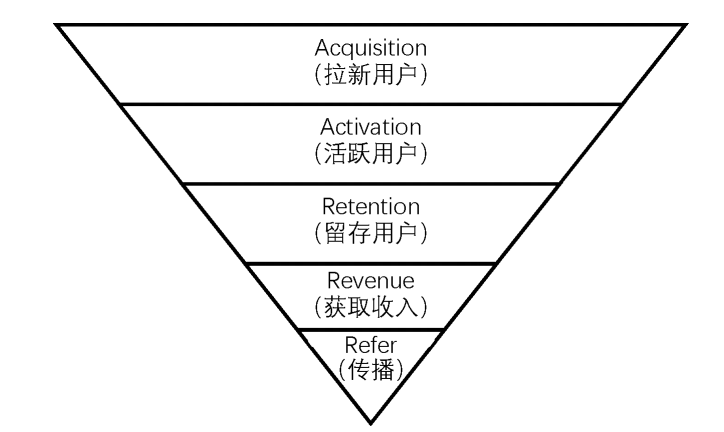
\includegraphics[keepaspectratio]{AARRR模型.png}}

}

\caption{AARRR MODEL}

\end{figure}%

\section{拉新指标}\label{ux62c9ux65b0ux6307ux6807}

是衡量新媒体广告投放效果的重要指标，主要包括CPM（Cost Per
Mill）、CPC（Cost Per Click）和CPA（Cost Per
Action）。这些指标帮助广告主评估广告投放的效率和效果，从而优化广告策略，提高投资回报率。

\subsection{CPM（Cost Per Mill）}\label{cpmcost-per-mill}

指每千次曝光的成本，它是衡量广告投放效率的重要指标，反映了广告主为每千次广告曝光所支付的费用。CPM越低，表示广告投放效率越高，广告主能够以更低的成本获得更多的曝光机会。

\subsubsection{计算公式：}\label{ux8ba1ux7b97ux516cux5f0f}

\[
\text{CPM} = \left( \frac{\text{总花费成本}}{\text{总曝光次数}} \right) \times 1,000
\]

\subsubsection{计算示例：}\label{ux8ba1ux7b97ux793aux4f8b}

假设一个广告活动的总花费成本为5000元，总曝光次数为200000次，那么CPM的计算如下：

\[
\begin{aligned}
\text{CPM} &= \frac{5,000}{200,000} \times 1,000 \\
           &= 0.025 \times 1,000 \\
           &= 25
\end{aligned}
\]

因此，该广告活动的CPM为25元，意味着广告主每获得1000次曝光需要支付25元的费用。

\subsection{CPC（Cost Per Click）}\label{cpccost-per-click}

指每次点击的成本，是衡量广告投放效果的重要指标，反映了广告主为每次用户点击所支付的费用。CPC越低，表示广告投放效率越高，广告主能够以更低的成本吸引更多的用户点击。

\subsubsection{计算公式：}\label{ux8ba1ux7b97ux516cux5f0f-1}

\[
\text{CPC} = \left( \frac{\text{总花费成本}}{\text{总点击次数}} \right) 
\]

\subsubsection{计算示例：}\label{ux8ba1ux7b97ux793aux4f8b-1}

假设你投放了一个网页广告，想吸引人进某个网站，总花费
3,000元，该网页广告总点击次数150次。那么CPC的计算如下：

\[
\begin{aligned}
\text{CPC} &= \frac{3,000}{150}  \\
           &= 20
\end{aligned}
\]

每吸引1个潜在用户点进网站，需要支付20元。

\subsection{CPA（Cost Per Action）}\label{cpacost-per-action}

指每次行动的成本，
计算逻辑是：总广告花费除以实际达成的行动（转换）次数。是衡量广告投放效果的重要指标，反映了广告主为每次用户完成特定行动所支付的费用。CPA越低，表示广告投放效率越高，广告主能够以更低的成本促使更多的用户完成特定行动。「行动」的定义由你決定，常見的包括：完成報名、购买產品、下载
App、填寫谘询表單等。

\subsubsection{计算公式：}\label{ux8ba1ux7b97ux516cux5f0f-2}

\[
\text{CPA} = \left( \frac{\text{总花费成本}}{\text{总转化次数}} \right)
\]

\subsubsection{计算示例：}\label{ux8ba1ux7b97ux793aux4f8b-2}

假设你举办了一場「线上讲座」，並透过广告导流报名： 总广告花费： 10,000
元，总点击数 (CPC 階段)： 500 次， 最终完成报名人数： 20 。

那么CPA的计算如下：

\[
\begin{aligned}
\text{CPA} &= \frac{10,000}{20}  \\
           &= 50
\end{aligned}
\]

每促成1个用户完成报名，需要支付50元的费用。这个CPA值可以帮助你评估广告投放的效果，并决定是否需要调整广告策略以降低CPA，提高转化率。

\subsection{三大指標比較表 (CPM / CPC /
CPA)}\label{ux4e09ux5927ux6307ux6a19ux6bd4ux8f03ux8868-cpm-cpc-cpa}

{\def\LTcaptype{none} % do not increment counter
\begin{longtable}[]{@{}
  >{\raggedright\arraybackslash}p{(\linewidth - 6\tabcolsep) * \real{0.2500}}
  >{\raggedright\arraybackslash}p{(\linewidth - 6\tabcolsep) * \real{0.2500}}
  >{\raggedright\arraybackslash}p{(\linewidth - 6\tabcolsep) * \real{0.2500}}
  >{\raggedright\arraybackslash}p{(\linewidth - 6\tabcolsep) * \real{0.2500}}@{}}
\toprule\noalign{}
\begin{minipage}[b]{\linewidth}\raggedright
指标
\end{minipage} & \begin{minipage}[b]{\linewidth}\raggedright
英文
\end{minipage} & \begin{minipage}[b]{\linewidth}\raggedright
核心关注点
\end{minipage} & \begin{minipage}[b]{\linewidth}\raggedright
范例
\end{minipage} \\
\midrule\noalign{}
\endhead
\bottomrule\noalign{}
\endlastfoot
CPM & Cost Per Mille & 品牌曝光 (被看見) & 花 1,000 元让 10,000
人看到 \\
CPC & Cost Per Click & 网站流量 (点進來) & 花 1,000 元換 100
个人進站。 \\
CPA & Cost Per Action & 最終转换 (留资料/買東西） & 花 1,000 元換 2
个人下單。 \\
\end{longtable}
}

\begin{tcolorbox}[enhanced jigsaw, arc=.35mm, bottomrule=.15mm, bottomtitle=1mm, breakable, colback=white, colbacktitle=quarto-callout-important-color!10!white, colframe=quarto-callout-important-color-frame, coltitle=black, left=2mm, leftrule=.75mm, opacityback=0, opacitybacktitle=0.6, rightrule=.15mm, title=\textcolor{quarto-callout-important-color}{\faExclamation}\hspace{0.5em}{Important}, titlerule=0mm, toprule=.15mm, toptitle=1mm]

CPA 最重要

\begin{itemize}
\item
  衡量真正的投资报酬率 (ROI)： 点击再多，如果没人买单也是徒劳。CPA
  直接告诉你获取一个客户的代价。
\item
  预算控制： 如果你知道一个学员的报名费是 3,000 元，而你的 CPA 是 500
  元，那你就能清楚算出利润空间。
\item
  优化转换率 (CVR)： 如果 CPC 很低（很多人进站）但 CPA
  很高（没人买），就代表你的网页内容或产品定价出了问题
\end{itemize}

\end{tcolorbox}

\section{活跃指标}\label{ux6d3bux8dc3ux6307ux6807}

\subsection{日活跃用户数（DAU, Daily Active
User)}\label{ux65e5ux6d3bux8dc3ux7528ux6237ux6570dau-daily-active-user}

表示在一天24小时内至少访问过一次网站或应用程序的\textbf{不重複用戶（Unique
Users）(独立用户)}數量。不管同一個用户在一天內進出網站多少次，DAU
都只會計算為 1。与此对应的，还有\textbf{周活跃用户数}(WAU, Weekely
Active User)与\textbf{月活跃用户数}(MAU, Monthly Active User)。

\subsection{用户黏着度（Stick
Rate）}\label{ux7528ux6237ux9ecfux7740ux5ea6stick-rate}

指用户在一定时间内的活跃程度，通常通过DAU（每日活跃用户数）与MAU（月活跃用户数）的比率来衡量。这个指标反映了用户对网站或应用程序的忠诚度和使用频率。用户黏着度越高，表示用户更频繁地使用该平台，说明平台具有较强的吸引力和用户粘性。

\[
\text{用戶黏著度(Stick Rate)} = \left( \frac{\text{DAU}}{\text{MAU}} \right) \times 100\%
\]

\subsubsection{舉例：}\label{ux8209ux4f8b}

如果某老师开设一门线上课程，有 100 名學生选修 (MAU =
100)。每天固定會上線看進度的學生有 20 名 (DAU = 20)，则黏著度：
\(20 / 100 = 20\%\)。

\subsection{PV(Page View)}\label{pvpage-view}

指页面浏览量，网页被「加载」或「刷新」的总次数。只要页面被读取一次，PV
就会加
1。衡量网站或应用程序的访问量。\ul{\textbf{\emph{每当用户访问一个页面时，PV就会增加一次}}}。PV是评估网站流量和用户兴趣的重要指标，通常用于分析网站的受欢迎程度和内容的吸引力。

计算逻辑： 不管是谁看的，只要有开启网页的动作就计算。
同一个使用者反覆刷新页面，PV 会不断累积。

\subsection{UV(Unique Visitor)}\label{uvunique-visitor}

指独立访客数(唯一页面浏览量)，在同一个工作阶段内，特定网页被浏览的「次数」。它排除了重复浏览，以「人（精确来说是浏览器/Cookie）」为单位。衡量在一定时间内访问网站或应用程序的独立用户数量。\ul{\textbf{\emph{每个独立用户只会被计算一次，无论他们访问了多少次}}}。UV是评估网站受众规模和用户覆盖范围的重要指标，通常用于分析网站的用户基础和市场渗透率。

计算逻辑： 同一个使用者在一次访问中，不管看几次同个页面，只算 1
次。能更准确地反映出「有多少人」看过这个内容。

\subsection{比较(PV;UV)}\label{ux6bd4ux8f83pvuv}

假设有一位学生进入某老师的课程网站，发生了以下行为：

1.进入 \texttt{首页\ (Home)}

2.点击进入 \texttt{课程大纲\ (Syllabus)}

3.按「重新整理」刷新 \texttt{课程大纲}

4.回到 \texttt{首页}

5.再次点进 \texttt{课程大纲}

統計結果如下：

{\def\LTcaptype{none} % do not increment counter
\begin{longtable}[]{@{}lll@{}}
\toprule\noalign{}
页面 & PV & UV \\
\midrule\noalign{}
\endhead
\bottomrule\noalign{}
\endlastfoot
首页 & 2 & 1 \\
课程大纲 & 3 & 1 \\
\textbf{总计} & \textbf{5} & \textbf{2} \\
\end{longtable}
}

这两个数字的「差距」能告诉你很多关于网页内容的信息：

\begin{itemize}
\tightlist
\item
  PV 远高于 UV：
\end{itemize}

---可能是好现象：
代表内容非常吸引人，使用者反覆回来查看（例如：参考资料、工具页面）。

---也可能是坏现象：
可能代表网页加载有问题、信息太复杂，导致使用者必须不断重新整理或来回跳转才能看清楚。

\begin{itemize}
\tightlist
\item
  PV 与 UV接近：
\end{itemize}

---代表使用者通常「看完就走」，没有回头再看的动力。




\end{document}
